\tikzstyle{inner} = [thin, circle, minimum size = 0.3cm, draw, inner sep = 0.1pt, black]
\tikzstyle{inner_g} = [thin, circle, minimum size = 0.3cm, draw, inner sep = 0.1pt, black, fill = green]
\tikzstyle{inner_r} = [thin, circle, minimum size = 0.3cm, draw, inner sep = 0.1pt, black, fill = red]
\tikzstyle{inner_b} = [thin, circle, minimum size = 0.3cm, draw, inner sep = 0.1pt, black, fill = blue!50!white]
\tikzstyle{ed} = [thick, ->, draw, black]

\begin{tikzpicture}
    
%    \draw[black, thick] (0.4, -0.4) rectangle (3.2, -1.6);
    \node at (-0.3, -1.2) {\scriptsize $X$};
    \node at (2, 0.3) {\scriptsize $Y$};
    \only<2>{
        \fill[green] (0, 0) rectangle (4, -2.4);
    }
    \only<3>{
        \fill[green] (0, -1) rectangle (4, -2.4);
    }
    \only<4>{
        \fill[green] (1.4, -1) rectangle (4, -2.4);
    }
    \only<5>{
        \fill[green] (1.4, -1) rectangle (2.4, -2.4);
    }
    \draw[step = 0.2, gray, thin] (0, 0) grid (4, -2.4);
    \draw[black, very thick] (0, 0) rectangle (4, -2.4);
    \only<3->{
        \draw[black, thick] (0, -1) -- (4, -1);
    }
    \only<4->{
        \draw[black, thick] (1.4, -1) -- (1.4, -2.4);
    }
    \only<5->{
        \draw[black, thick] (2.4, -1) -- (2.4, -2.4);
    }
    \only<5>{
        \node[black, fill = green, rounded corners = 5pt] at (1.9, -1.7) {$t_2$};
    }
\end{tikzpicture}